\section*{\center Evaluación continua del tema 1}
\subsection*{\center Análisis de datos en R}
\vspace{2cm}

\begin{multicols}{2}

\subsubsection*{Introducción}
Se extrajo la información del sitio oficial del instituto nacional de estadística (INE) de Bolivia.\\\\
Para la primera sección, se tomo una encuesta de hogares \href{http://anda.ine.gob.bo/index.php/catalog/88/get-microdata}{http://anda.ine.gob.bo/index.php/catalog/88/get-microdata}. La encuesta fue realizada en el año 2020, con el objetivo de conocer la percepción de los hogares de la población Boliviana. Más específicamente, la educación en dicho país.\\\\
Para la segunda sección (series temporales) se tomo datos de \href{http://anda.ine.gob.bo/index.php/catalog/11/get-microdata}{http://anda.ine.gob.bo/index.php/catalog/11/get-microdata} donde se estudiara estadisticas e indicadores de hidrocarburos para los años  1990 al 2017.\\\\

\end{multicols}

\vspace{.5cm}

\subsection*{\center Educación en Bolivia}

\begin{multicols}{2}

\subsubsection*{Pregunta de la investigación}
\begin{center}
    \begin{itemize}
	\item ¿Qué proporción de grados de estudio tienen los encuestados?
	\item ¿Qué proporción de hombres y mujeres mayores de 18 años en función de la edad no fue a la escuela o no concluyeron satisfactoriamente el bachillerato?
	\item ¿Cuál es la diferencia de salarios líquidos excluyendo descuentos que tiene los encuestados según el grado de estudios?
    \end{itemize}
\end{center}

\subsubsection*{Análisis univariante para la edad}
La media de edad de la encuesta realizada fue de \textbf{30 años}, con una desviación estándar de \textbf{21 años} y un coeficiente de variación de \textbf{0.7}\\\\
La curva de densidad para las edades de la encuesta fue:
\begin{center}
    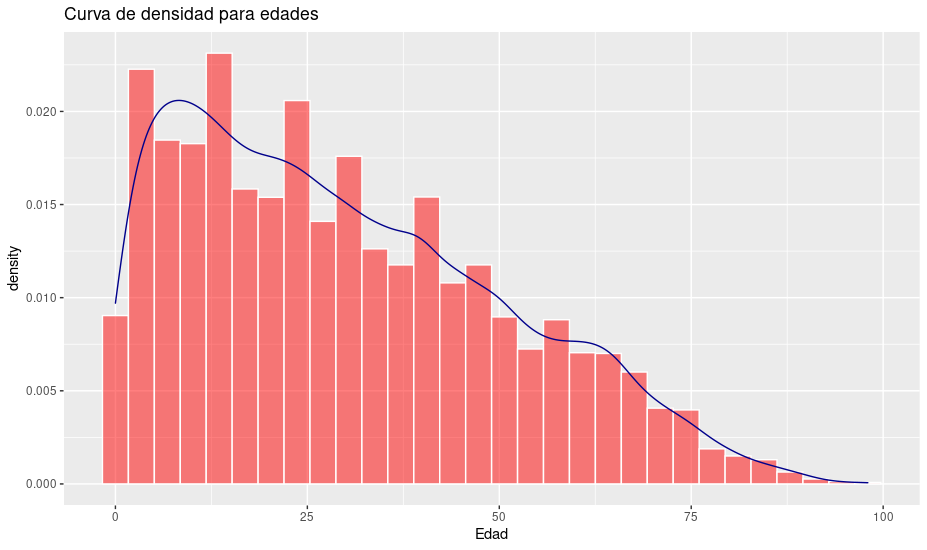
\includegraphics[scale = 0.32]{codigoFuente/tareas/estadistica/imagenes/densidad_edad.png}
\end{center}
Teniendo en cuenta que en promedio una persona acaba el bachillerato  aproximadamente a los 18 años entonces concluimos que, 
\begin{center}
    \begin{tabular}{|c|c|c|c|c|c|}
	\hline
	Sin&no&&nivel&&post-\\
		     educa&bachiller&bachiller&técnico&grado&grado\\
		     \hline
			  2467&15031&9047&1386&6334&354\\
			  \hline
    \end{tabular}
\end{center}

\begin{center}
    \begin{tabular}{|c|c|c|c|c|c|}
	\hline
	Sin&no&&nivel&&post-\\
		     educa&bachiller&bachiller&técnico&grado&grado\\
		     \hline
			  6.6\%&40.5\%&24.3\%&3.7\%&17\%&0.9\%\\
			  \hline
    \end{tabular}
\end{center}

De donde podemos inferimos que el $40\%$ no concluyeron el bachillerato, el $24\%$ concluyeron el bachillerato , el $17\%$ concluyeron el grado y menos del $1\%$ realizo y concluyo un doctorado.\\\\

\subsubsection*{Análisis bivariante para el género y edad}
Empezamos construyendo intervalos de 10 años de edad. Para la cual tenemos la siguiente tabla. 
\begin{center}
    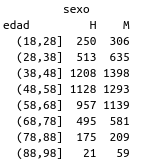
\includegraphics[scale = 0.6]{codigoFuente/tareas/estadistica/imagenes/tabla1.png}
\end{center}

Sacando la proporción por columna,\\
\begin{center}
    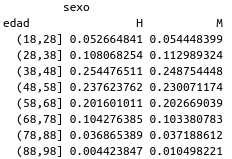
\includegraphics[scale = 0.6]{codigoFuente/tareas/estadistica/imagenes/tabla3.png}
\end{center}

Y sabiendo que en edad promedio una persona se gradúa del bachillerato a los 18 años, por lo que se filtro a personas menores a 18, llegamos a la conclusión de que $25\%$ de los hombres y el $24\%$ de las mujeres entre los 38 y 48 años no fue a la escuela o no concluyo el bachillerato.\\\\

\subsubsection*{Regresión simple}
Al realizar un modelo de regresión lineal, entre los salarios líquidos y el grado de educación,
\begin{center}
    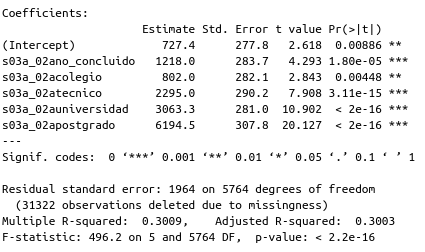
\includegraphics[scale = 0.6]{codigoFuente/tareas/estadistica/imagenes/reg_simp.png}
\end{center}
vemos que la diferencia entre los salarios líquidos de una persona que no asistió a la escuela son menores en 1218 Bolivianos (moneda Boliviana) a la que si asistió pero no termino el bachillerato, son 3063 bs menores a los que fueron concluyeron la universidad y 6194 bs menores a los que concluyeron un postgrado.\\\\

\subsubsection*{Regresión multiple}
Realizando un modelo de regresión multiple, entre salarios líquidos y el grado de educación mas el género,
\begin{center}
    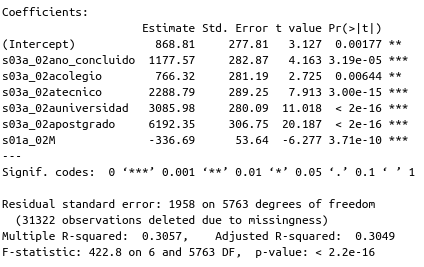
\includegraphics[scale = 0.6]{codigoFuente/tareas/estadistica/imagenes/reg_mult.png}
\end{center}

Y similar a al modelo anterior podemos señalar que los que no concluyeron el bachillerato pero si asistieron a la escuela, ganan en promedio 1177 Bs. mas que los que no fueron a la escuela, los técnicos superiores 1622 Bs. mas que los que acabaron el bachillerato (2288 Bs. - 766 Bs.). 
\\ Las mujeres ganan 336 en moneda Boliviana menos que los hombres.
\end{multicols}
\newpage
\subsection*{\center Producción de gas natural (1990-2017)}

\begin{multicols}{2}
\subsubsection*{Pregunta de la investigación}
\begin{center}
    \begin{itemize}
	\item ¿Cómo varia la producción de gas natural cada mes año tras año?
	\item ¿Cual es el aumento de producción cada año desde 2000 hasta 2017?
    \end{itemize}
\end{center}

\subsubsection*{Análisis de series temporales}
\begin{center}
    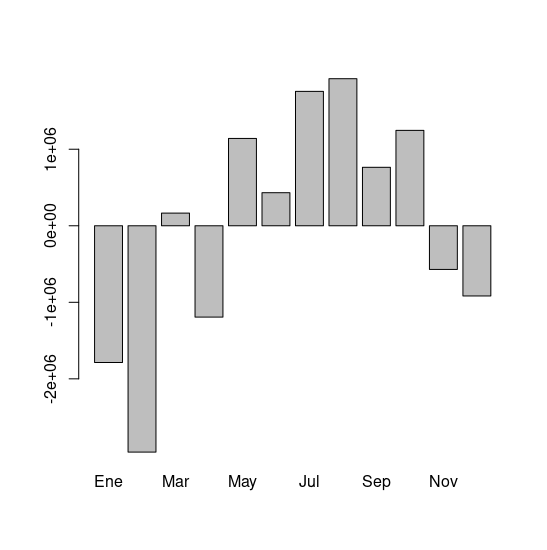
\includegraphics[scale = 0.6]{codigoFuente/tareas/estadistica/imagenes/descom.png}
\end{center}
Realizando una descomposición aditiva como la anterior figura,
vemos que los cuatro primeros meses año tras año la producción de gas natural es menores que la media, para luego tener un realce mayor a la media entre mayo y octubre y una atenuación menor a la media para noviembre y diciembre. \\\\

Para responder a la segunda cuestión suavizamos la serie temporal en medias móviles de orden 5 en el periodo 2000-2017 y aplicamos el modelo de regresión lineal simple como se muestra en la figura siguiente,

\begin{center}
    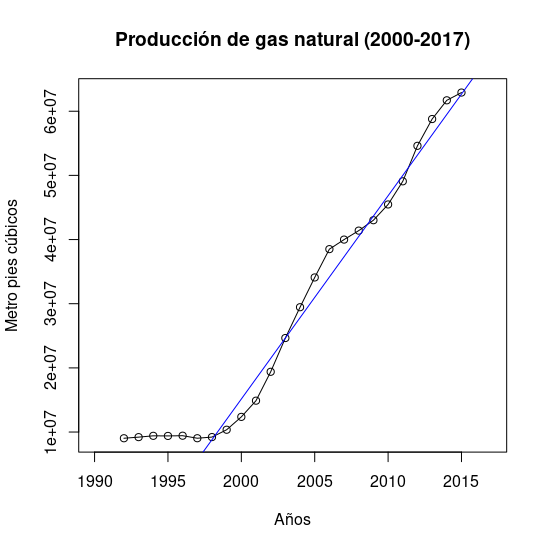
\includegraphics[scale = 0.5]{codigoFuente/tareas/estadistica/imagenes/st.png}
\end{center}

En conclusión vemos que la producción de gas natural aumenta de año en año, es decir, la producción de gas natural aumenta en $3.16\cdot 10^6$ metro pies cúbicos.\\\\

\end{multicols}
